\section{State Of The Art}

\subsection{Monitoring using Video or Audio}
\label{chap21}
Current smart home environments consist of several appliances and other devices, with sensors, actuators and/or biomedical monitors. These systems are used by the residents in a daily basis. In some situations the house is monitored using video and audio technologies, even tho they present some disadvantages like: high costs due to sophisticated equipments and specialized deployment, the need for a large bandwidth or privacy issues. 
Several state-of-the-art solutions were reviewed. In \cite{2} falls are detected. In order to reduce the number of false alarms, the system integrates a \acs{WSN} and a video system. Cameras activated by a wireless sensor tracking mechanism, are able to interpret the video signal and make decisions whether to call an emergency number or not. A voice communication \acs{IEEE} 802.15.4 is also discussed through the usage of state-of-the-art radios capable of transmitting voice.\\
In \cite{3} and \cite{4} an installed surveillance system is used to infer about the position of a resident. No interaction with the system is needed in order to locate the person. The usage of \textit{Smart Cameras} allows to resolve the privacy issue of data transmission through air, with the possibility of spoofing, which would present serious security concerns to the user.\\
\cite{5} deploys another monitoring application in a care home. It refers to the need for more healthcare professionals and the small amount of time that each one of them has available for each elder. The volume of biomedical data gathered can improve the way that the case manager follows it's dependent.\\
\cite{6} refers to the term \textit{aging in place} which represents a movement where elders live in an independent and safe manner in their own homes. Monitoring of falls but also utilitarian functionalities are implemented such as object detection, calendar, video-conference and address book.\cite{7} uses video and audio to correctly deduce if a fall has happen.
%%%%%%%%%%%%%%%%%%%%%%%%%%%%%%%%%%%%%%%%%%%%%%%%%%%%%%%%%%%%%%%%%%%%%%%%%%%%%%%%%%%%%%%%%%%%%
%%%%%%%%%%%%%%%%%%%%%%%%%%%%%%%%%%%%%%%%%%%%%%%%%%%%%%%%%%%%%%%%%%%%%%%%%%%%%%%%%%%%%%%%%%%%%
%%%%%%%%%%%%%%%%%%%%%%%%%%%%%%%%%%%%%%%%%%%%%%%%%%%%%%%%%%%%%%%%%%%%%%%%%%%%%%%%%%%%%%%%%%%%%

\subsection{Monitoring using Wearable Sensors}
\label{chap22}
The reduction in size of wireless sensors is bringing to the market solutions that can track a person's health, independently of his location or activity. The possibility of smart clothes with built-in sensors sufficiently small and light to be carried without any discomfort, enable the mass usage of such equipments in a medium term.
In \cite{8} the \acf{BSN} is addressed, as a solution to early detect heart problems with sensors capable of measuring temperature, acceleration or building an electrocardiogram, all connected to a central coordinator node using Bluetooth (Figure \ref{fig:4:bsn}).
\cite{9} discusses the the need for three types of priorities for messages in a \acs{WBAN}: \textit{On-demand} requested by a doctor or physician, in order to monitor the patient vital signs, \textit{Emergency} initiated by the sensors when some critical threshold has been exceeded and \textit{Normal} with the lowest priority.In \cite{10} it is discussed the problems that arise from the usage of Zigbee in a crowed \acs{WLAN} environment. An algorithm is suggested to solve this issue in which the Zigbee forces an \acs{AP} to leave from an occupied frequency.

\begin{figure}[!htb]
  \centering
  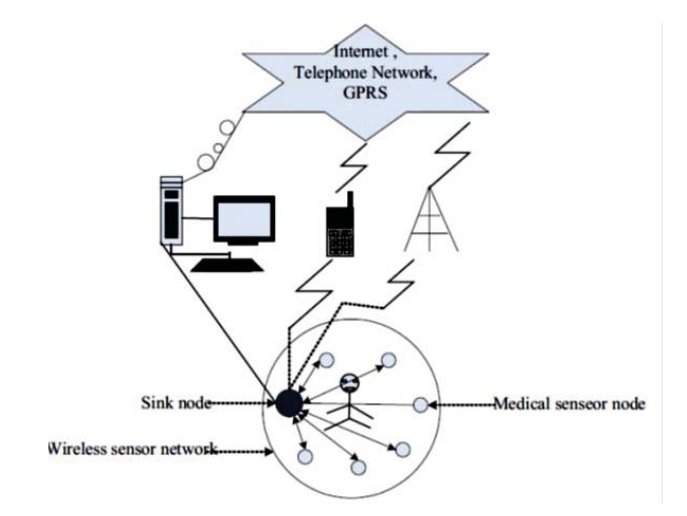
\includegraphics[width=0.30\textwidth]{img/02_body_sensor_network.png}
  \caption{Example of a Body Sensor Network (BSN)\cite{8}.}
  \label{fig:4:bsn}
\end{figure} 

\cite{11} suggests the integration of several networks into one integrated platform able to track a person in the interior or exterior enabling all the case managers to be constantly aware of their patient. The same paper also refers the need to develop sensors that don't present any discomfort to their users, since that might be a very strong reason for not wearing sensors during a long period of time.

%%%%%%%%%%%%%%%%%%%%%%%%%%%%%%%%%%%%%%%%%%%%%%%%%%%%%%%%%%%%%%%%%%%%%%%%%%%%%%%%%%%%%%%%%%%%%
%%%%%%%%%%%%%%%%%%%%%%%%%%%%%%%%%%%%%%%%%%%%%%%%%%%%%%%%%%%%%%%%%%%%%%%%%%%%%%%%%%%%%%%%%%%%%
%%%%%%%%%%%%%%%%%%%%%%%%%%%%%%%%%%%%%%%%%%%%%%%%%%%%%%%%%%%%%%%%%%%%%%%%%%%%%%%%%%%%%%%%%%%%%

\subsection{Monitoring using domestic sensors}
\label{chap23}
In this type of monitoring, information is gathered anonymously, using sensors with very minimal computational capabilities. Proximity sensors or sensors installed in home appliances are accessed in order to understand if the person is at home or has passed through a certain corridor. This type of monitoring has less granularity, which can be a problem if more information is needed.\cite{13} uses pressure sensors to help Alzheimer's patients reaching their destination inside house through the use of TV screens. \textit{MediaCup} is introduced in \cite{12} as fully ubiquous device. With a battery capable of charging using an electromagnetic field, the \textit{MediaCup} is fully hidden from user and coupled with a few sensors that can track, for instance, movement or acceleration (

\begin{figure}[!htb]
  \centering
  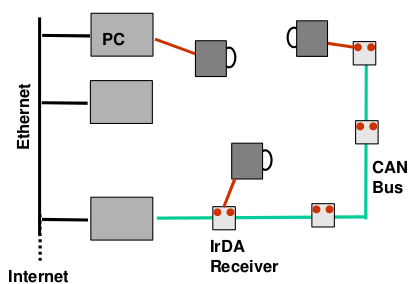
\includegraphics[width=0.40\textwidth]{img/02_mediacup.png}
  \caption{\textit{Mediacup}\cite{12} network infrastructure with IR, LAN and CAN.}
  \label{fig:6:mediacup}
\end{figure}

A lot of research has been done focusing falls, vital signs tracking and ubiquous computing. The recent development in \acp{BSN}s has brought to the scene new sensors and new concepts that can even be used for entertainment. Also the need for unobtrusive equipments and the lack of privacy of devices that store too much information, like cameras is a problem to be discussed. 

\section{Related Work}

\subsection{Elder Home Monitoring}
\label{chap31} 
In a study named \``The Activities of Daily Living Study''\ presented at \cite{16} several questionnaires were delivered to \acfp{CM} ( professionals that give assistance to elder people living at home). This study refers to the existence of a group of \acfp{ADL} which \acp{CM} keep track. These include getting up in the morning, dressing or feeding. Through these \acp{ADL} healthcare professionals are able to keep track of their elders mental and physical state. This study also sets some of the most valuable features which a monitoring system can present to elders. Features like panic buttons and security improvement measures seem to have success while others like cameras don't seem as accepted.\\
The study also enumerates some of the main needs in monitoring elder people in-home. Location tracking to know if the elder got up of his bed, better scheduling of visits as the \acs{CM} would be able to know if the elder is at home, house occupancy to understand the elder need for companionship.

\subsection{Position tracking for Wireless Sensor Networks}
\label{chap32} 
Several types of metrics allow for an inference of position. \acf{TOA}, \acf{TDOA}, \acf{RSS}, \acf{POA} and \acf{AOA}. \acs{TOA} and \acs{TDOA} are time based metrics and need expensive hardware and also constant synchronization between nodes. \acs{AOA} and \acs{POA} are angle and phase metrics in-home tracking is difficult due to shadowing and fading effects.\acs{RSS} is received power based. The number of distinct systems for location tracking is quite large, so the need to make choices at this stage arises.\\
The chosen system should be for a medium area using \acs{RF} due to the fact that some places in a home don't have line of sight, should use the received signal power \acs{RSSI}, should use a lookup table since that a model for the signal propagation inside a house is difficult to attain and varies from house to house and with position tracking centralized due to the computation constraints needed for accurate position tracking. Several algorithms that fit these characteristics were found. Namely two deterministic, RADAR \cite{28} with a 50\% 2.94 m precision and MoteTrack \cite{29} with a 50\% 2 m precision and one probabilistic, the HORUS \cite{31} which uses density probability functions to choose a position. All of these have offline moments, when a radio map is collected. In the online phase the information gathered in a radio map is then used to infer the position from a live sample.


\subsection{Routing protocols for Wireless Sensor Networks}
\label{chap33}
Several types of routing protocols exist for \acp{WSN}. They are divided in three main types: flat-routing, hierarchical-routing and location-based routing. In flat-routing all the nodes have the same capabilities and functionality. Existing protocols like the \acf{SPIN} \cite{20}, \acf{DD} \cite{21} and \acf{AODV} \cite{22} are all flat-routing. All of them do some kind of sensing to the network before actually sending a message. 

\begin{figure}[!htb]
  \centering
  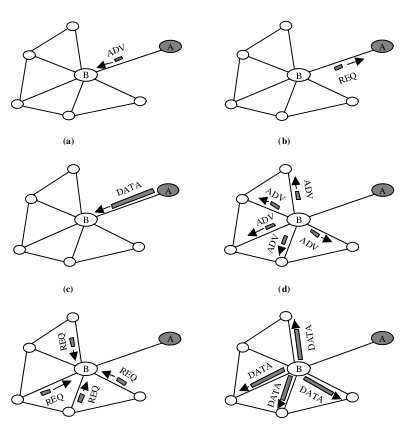
\includegraphics[width=0.39\textwidth]{img/03_spin.png}
  \caption{SPIN protocol example \cite{20}.}
  \label{fig:1:spin}
\end{figure}

\acs{SPIN} (Figure \ref{fig:1:spin}) implements the use of three types of messages: ADV (\textit{advertisment}), REQ (\textit{request} e DATA. Node A wants to send a message for one of the nodes connected to  B, so it sends an ADV to B (a). B is ready to receive and sends back to A a REQ (b). A receives it and sends DATA to B (c). B continues the process to send the message to it's coordinated nodes.
\acs{DD} uses gradients to find the best path and \acs{AODV} uses also a set of messages that allows it to find the best suitable path.\\
\acf{LEACH}\cite{24} and \acf{PEGASIS}\cite{25} are both hierarchical protocols and use the clusters concept to reduce the number of nodes that communicate with a base station. In \cite{26} \acf{GEAR} is presented as location-based protocol it's used in large deploy areas where the need for messages location sending is needed.

\section{Work Environment}


\begin{figure}[!htb]
  \centering
  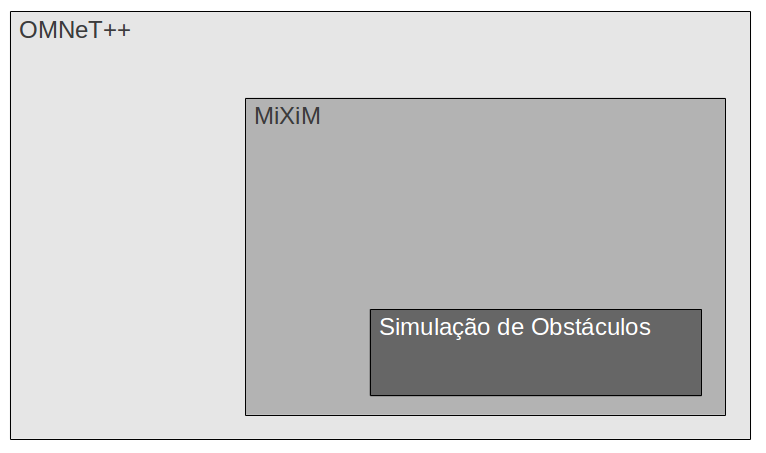
\includegraphics[width=0.35\textwidth]{img/04_framework_overview.png}
  \caption{Modular overview of the work environment.}
  \label{fig:1:frameworkOverview}
\end{figure}
Due to cost reasons the work presented in this paper was implemented using a simulated environment. The need to find a solution that would present close to real values and close to real behaviours, brought the need to use  \acf{OMNeT++}\cite{33}, the base framework and \acf{MiXiM}\cite{34}, a framework for \acs{OMNeT++} with mobility, channel and wireless sensors simulation great capabilities. Some of the reasons that make OMNeT++ the most obvious choice are: the modular hierarchical design, which can be combined for reuse and flexibility, the Object Oriented approach, the C++ internal structure, \acf{NED} language for module building and a auto-animated environment. \acs{MiXiM} in turn provides a complex channel losses model, which for indoor environments allow us to achieve close to real values and several \acs{MAC} and \acs{NIC} models for the \acs{IEEE} 802.15.4. Finally the simulation of obstacles was obtained using a \acs{MiXiM} modification \cite{35} that implements a simple obstacle model given by:
\begin{equation}
	L_{obs}[dB] = \beta{n} + \gamma{d_m}
\end{equation}
with attenuation per wall \begin{math}\beta{n}\end{math} and attenuation per meter \begin{math}\gamma{d_m}\end{math}, configurable using a XML file. 

In this work the following values were used:

\begin{table}[!htb]
	\centering
\begin{tabular}{ |c|c|c|}
	\hline
  	Profundidade(cm) & \begin{math}\beta{}\end{math}(dBm)  & \begin{math}\gamma{}\end{math}(m)\\
  	\hline
  	20 & 106.3 & 0 \\
  	10 & 26.575 & 0 \\
  	\hline
\end{tabular}
	\caption{}
	\label{tab:1:attenuationValues}
\end{table}

\section{System Architecture}

\subsection{Elder Monitoring System {EMoS}}
\begin{figure}[!htb]
  \centering
  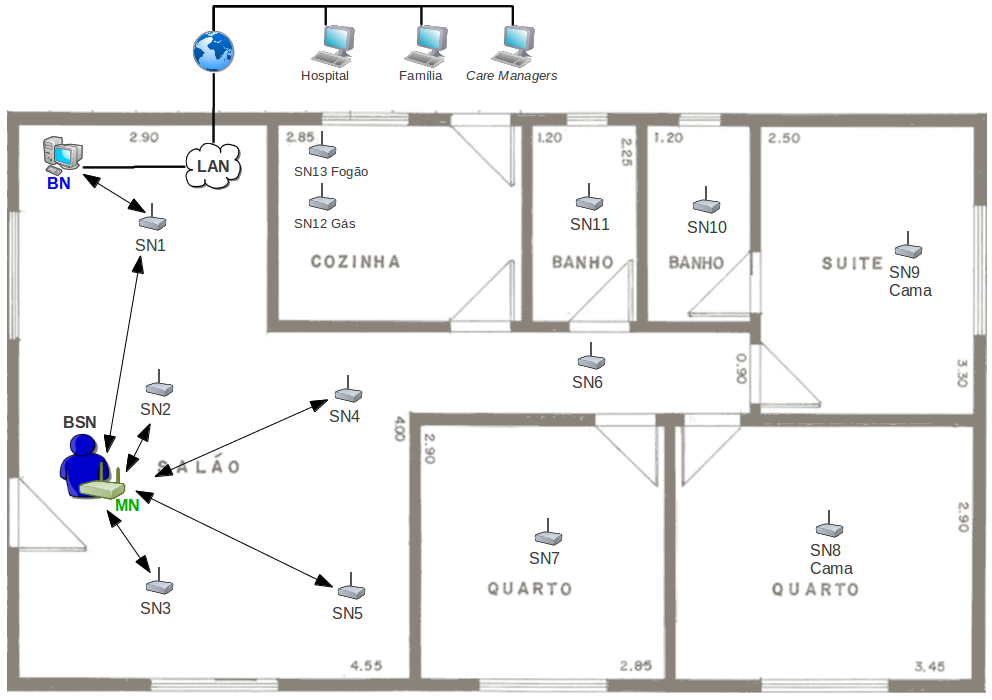
\includegraphics[width=0.47\textwidth]{img/05_emos_overview.png}
  \caption{Model structure of the \textit{Elder Monitorization System} (EMoS).}
  \label{fig:1:emosOverview}
\end{figure}
\acs{EMoS} is comprised of three types of nodes: \acf{SN}, \acf{MN} and \acf{BN}. These nodes all have distinct roles in the network.\\ The MN is a sensor equipped with two radios, one IEEE 802.15.4 and another Bluetooth for connecting with a BSN. It can be installed in a walker or a wheelchair. It has the ability to communicate with all the other nodes in the WSN and to record static node signatures for localization tracking.\\
The SN is a sensor equipped with one radio IEEE 802.15.4 capable of sending messages when connected to a stove or a bed pressure sensor and establishing communication with all the other nodes in the WSN. All static nodes are connected to the power network and don't need any batteries.\\
The BN is a USB IEEE 802.15.4 gateway and is connected to a PC. It has the  computational capability in the network. It is responsible for coordinating all the WSN, communications with the exterior and tracking all the mobile nodes detected.

All nodes share the same CSMA MAC layer and have an AODV custom build for this simulation Network Layer. The application layer differs accordingly to the node role.

\begin{figure}[!htb]
  \centering
  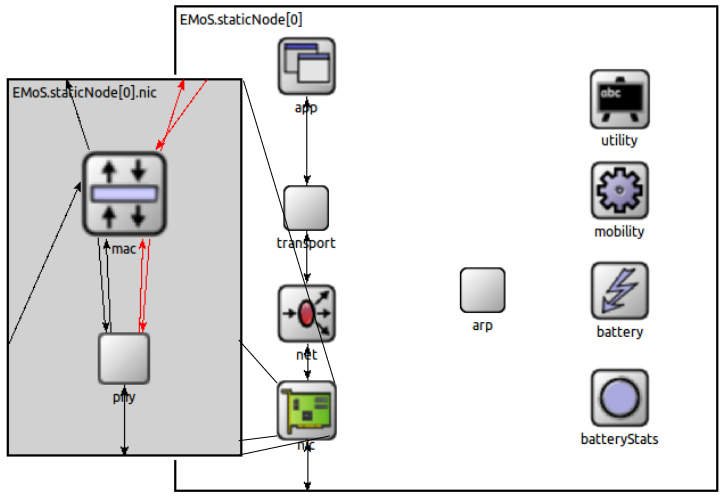
\includegraphics[width=0.40\textwidth]{img/05_emos_node_internal.png}
  \caption{Internal structure of a EMoS node.}
  \label{fig:2:emonsNodeInternal}
\end{figure}

Two types of radios exist in the simulation: the \textit{Texas Instruments CC 2420} and the \textit{Digi XBee}, with the following parameters, which are used to configure the NIC in each node:

\begin{table}[!htb]
	\centering
\begin{tabular}{ |l|r|}
	\hline
  	Par�metro & Valor \\
  	\hline
  	Modulation & O-QPSK \\
  	Receiver Sensitivity & -92 dbM  \\
  	Transmit Power	& 1mW \\
  	Sleep Current & <10 uA \\
  	Current Consumption RX & 50 mA \\
  	Current Consumption TX (P=0dBm) & 45 mA \\
  	\hline
\end{tabular}
	\caption{Radio \textit{Digi XBee}.}
	\label{tab:1:xbeeNICParameters}
\end{table}

\begin{table}[!htb]
	\centering
\begin{tabular}{ |l|r|}
	\hline
  	Par�metro & Valor \\
  	\hline
  	Modulation & O-QPSK \\
  	Receiver Sensitivity & -95 dBm  \\
  	Transmit Power & 1.1mW \\
  	Sleep Current & 0.02 uA \\
  	Current Consumption RX & 18.8 mA \\
  	Current Consumption TX (P=0dBm) & 17.4 mA \\
  	\hline
\end{tabular}
	\caption{Radio \textit{Texas Instruments CC2420}.}
	\label{tab:2:CC2420NICParameters}
\end{table}


\subsection{Network Layer}
The network layer is common to all nodes in the network. It has been implemented with an \acf{AODV} routing protocol which uses three types of messages for establishing the routes: \acf{RREQ}, \acf{RREP} and \acf{RERR}.\\ When a node A wants to communicate with a node B it sends the package from the application layer to the network layer. After arriving there it checks if there is a path to node B. If the path doesn't exist it sends a RREQ in broadcast mode to all the nodes. Each node knows if it has already forwarded a RREQ so that the same RREQ can only be sent by each node one single time. Each node that the RREQ passes creates a reverse route to the node A. When it reaches the destination, B sends a RREP through the reverse path created, using a unicast mode. As the RREP transverses the reverse path a forward path to node B is created. When node A receives the RREP it gets the waiting packet and sends it to the B trough the new path found.\\
Finally, when a message cannot be delivered the node that detected the route failure, sends a RERR to all the route precursors (nodes that used the route before it failed). This information removes the route and makes node A to send a RREQ again.\\
In EMoS this schema was fully implemented and only the local-repair function was left out.

\subsection{Application Layer}
\begin{figure}[!htb]
  \centering
  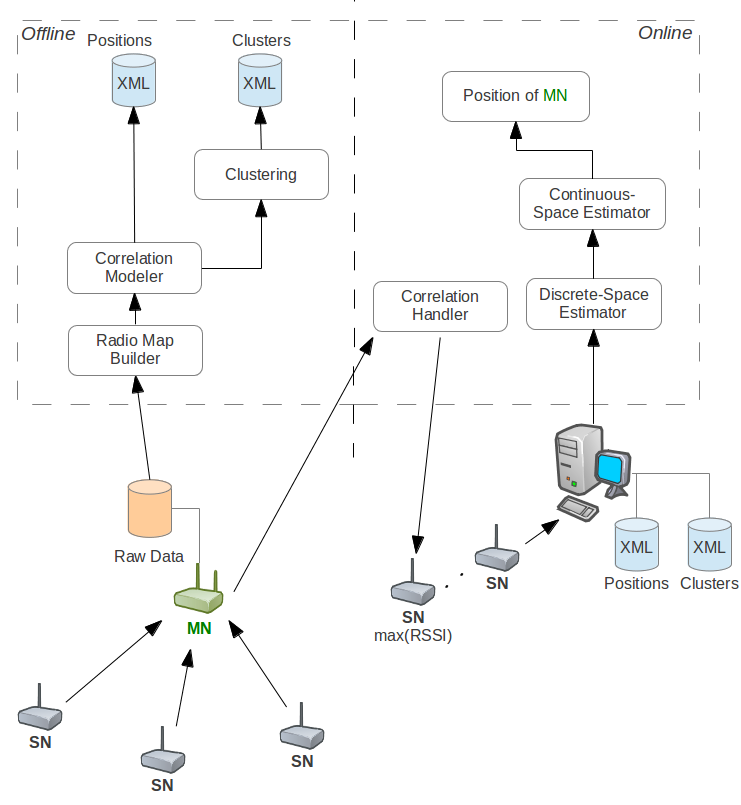
\includegraphics[width=0.48\textwidth]{img/05_horus_mod.png}
  \caption{Modified HORUS modules.}
  \label{fig:17:horusMod}
\end{figure}
Although each node is capable of sending messages from the application layer, the most important feature, is the position tracking which will be the focused in this paper.

The position tracking in EMoS is made using a modified versions of HORUS\cite{31}. It uses a probabilistic method which uses probabilistic density functions in it's parametrized form, to calculate the probability of a mobile node being in a certain position. The HORUS has two phases. An offline phase where a radio map is built and a online phase where the built radio map is used to infer the position of the mobile node.\\
In the offline phase MN is in calibration mode what means that it will capture all the static nodes signatures till a position change occurs. In this process it stores in a \textit{Raw} database all the signatures collected.The data is then transformed in radio ma positions in which for each position and each node the mean and standard deviation is found using the following equations:

\begin{equation}
\mu{} = \frac{1}{n}\sum_{j=1}^{n} s_i(j)\
\label{eq2}\
\end{equation}

\begin{equation}
\sigma{} = \sqrt{\frac{1}{n}\sum_{j=1}^{n}(s_i(j)-\mu{})^2}
\label{eq3}
\end{equation}

These two values are used in the normal probability density function:

 \begin{equation}
pdf(q) = \frac{1}{\sigma{}\sqrt{2\pi{}}}e^\frac{-(q-\mu)^2}{2\sigma{}^2}
\label{eq1}
\end{equation}

For each position a set of static nodes addresses are stored together with their correspondent mean and standard deviation. This results in a normal distribution for each static node in each position. The parametrization of the distribution allows for a filtering of erroneous values and existence of values for all the signal strength range.

\begin{figure}[!htb]
  \centering
  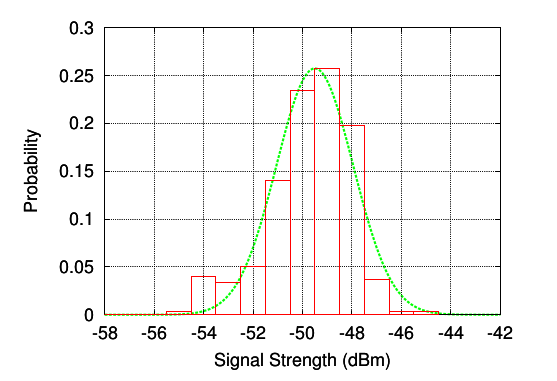
\includegraphics[width=0.48\textwidth]{img/05_horus_normal.png}
  \caption{Parametrized probability density function \cite{31}.}
  \label{fig:23:horusNormal}
\end{figure}

In EMoS this information is stored in a XML file. After this process the result is sent to the Clustering model which divides all the positions in clusters. The division is made using the position key determined by the 2 largest signal strength value nodes.

In the online phase the MN collects all the signatures during a certain amount of time. When that time is over it calculates the mean signal strength for each static node received and sends the result to the closest SN. 

The SN in turn sends to the BN (Base Node). Note that if no route is available the network layer will find one using AODV. When the message with the static nodes samples arrives to the BN it will be used to infer the MN position. This will be made using firstly a discrete-space estimator and afterwords a continuous-space estimator. The discrete-space estimator can only determine a position available in the radio map while the continuous-space estimator allows all the other points.

All correlation modules are simple mean operations.

Therefore when the message arrives to the discrete-space estimator it's joint probability is calculated as:

\begin{equation}
P = \prod_{j=1}^{n} P_i
\end{equation}

where \begin{math}P_i\end{math} is:

\begin{equation}
P(s_i<=0.5) = P(Z<=\frac{s_i+0.5-\mu{}}{\sigma{}_i})
\end{equation}

The position with the largest probability wins and is considered the position where the mobile node is. But, because the discrete-space estimator only allows the positions stored in the radio map it is necessary to use the continuous-space estimator to improve the accuracy of the estimated value.

Two techniques are applied: Center of mass of the positions and Time-averaging in the physical space.  

The first uses the other smaller probabilities calculated to triangulate a new position, using the following equations:

\begin{equation}
x = \frac{\sum_{j=1}^{min(N,P)} x_iP_i}{\sum{}P_i}
\end{equation}
\begin{equation}
y = \frac{\sum_{j=1}^{min(N,P)} y_iP_i}{\sum{}P_i}
\end{equation}

The second uses previous stored estimated positions to get a mean value of the new position:

\begin{equation}
x = \frac{\sum_{j=1}^{K} x_i}{K}
\end{equation}
\begin{equation}
y = \frac{\sum_{j=1}^{K} y_i}{K}
\end{equation}

This makes a reasonable approach to the real positions. HORUS authors affirm to get 0.86 m in 90\% of the cases in a real test-bed.